\section{Theorie}
\label{sec:Theorie}
Mittels der Kernspinresonanz
können ein Teil der magnetische Momente von Atomkernen
in einer Probe
durch Anlegen eines
äußern Magnetfeldes
gezielt verändert werden und somit
eine makroskopische Magnetisierung der Probe
erzeugen.
Durch die Kernspinresonanz ist es möglich
Aussagen zur Molekülstruktur wie z.B. chemischen Bindungen
zu machen.
Des Weiteren  können auch mikroskopische
Relaxationsprozesse innerhalb der Probe
durch Anlegen eines
äußern magnetischen Wechselfeldes
untersucht
werden.


% Einleitung
% kurze zusammen fassung kernspinresonaz
\subsection{Kernspinresonaz}
Zunächst soll die Magnetisierung einer Probe
in einem Magnetfeld $\vec{B}=B_0\vec{e}_z$,
die sich im thermischen Gleichgewicht befindet, betrachtet werden.
Durch den Zeeman-Effekt
spalten sich die Kernspinzustände mit
Spinquantenzahl $I$ in
 $2I+1$ äquidistante Unterniveaus auf.
 Die Unterniveaus werden mittels
 der Orientierungsquantenzahl $m$
$(-I \leq m \leq I)$ unterschieden und
benachbarte Niveaus besitzen die Energiedifferenz
\begin{align*}
  \Delta E =\gamma B_0 \hbar.
\end{align*}
Die Besetzung im thermischen Gleichgewicht
bei der Temperatur $T$ erfolgt nach der
Boltzmann-Verteilung. Es folgt demnach
für das Besetzungsverhältnis zweier benachbarter Niveaus
\begin{align}
  \frac{N(m)}{N(m-1)} &= \exp\left(-\frac{\gamma B_0 \hbar }{k_B T}\right).
\intertext{Durch die ungeleiche Besetzung
ergibt sich eine Kernspinpolarisation}
\langle I_z \rangle &= \frac{\sum_{m=-I}^{m=I}\hbar m \exp\left(-\frac{m\gamma B_0 \hbar}{k_B T} \right) }{\sum_{m=-I}^{m=I}\exp\left(-\frac{m\gamma B_0 \hbar}{k_B T}\right)}. \label{eqn:I_z}
\end{align}

Werden nur Protonen betrachtet, ergibt
sich, da $I=\tfrac{1}{2}$
eine Aufspaltung, die in der
Abbildung \ref{fig:Proton} dargestellt ist.

\begin{figure}
 \centering
 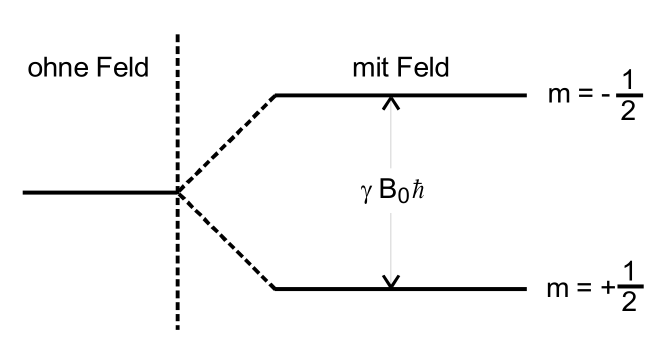
\includegraphics[width=0.5\textwidth]{Zeeman.PNG}
 \caption{Aufspaltung der Energieniveaus im Magnetfeld $B_0$ für $I=\tfrac{1}{2}$.\cite{sample}}
 \label{fig:Proton}
\end{figure}
Für Zimmertemperatur und Magnetfelder
der größenordnung $\SI{1}{\tesla}$
gilt $m\gamma B_0 \hbar \ll k_BT$.
Die Kernspinpolarisation für Proton
vereinfacht sich
durch die Näherung zu
\begin{align}
\langle I_z\rangle_P= -\frac{\hbar^2}{4}\frac{\gamma B_0}{k_B T}.
\end{align}
Für die Gleichgewichtsmagnetisierung $M_0$ bei der
der Temperatur $T$ in $\vec{e}_z$-Richtung gilt dann
\begin{align}
M_0=\frac{1}{4}\mu_0 \gamma^2 \frac{\hbar^2}{k_B} N \frac{B_0}{T}
\end{align}
mit $N$ der Anzahl der Momente pro Volumeneinheit.

\subsection{Larmor-Präzession}
\label{subsec:Larmor}
Durch die große Anzahl von Einzelmomenten in einer Probe \approx $\SI{10e28}{\per\cubic\meter}$
kann die Probenmagnetisierung $\vec{M}$ mit klassischen Methoden
beschrieben werden.
Auf eine Magnetisierung $\vec{M}$ in einem Feld $B_0\vec{e}_z$
wirkt somit ein Drehmoment
\begin{align}
\vec{D}=\vec{M} \times \vec{B}_0 \vec{e}_z
\end{align}
und gemäß der Kreiselgleichung
\begin{align}
  \frac{\symup{d}\vec{I}}{\symup{d}t}=\vec{M}\times\vec{B}_0 \vec{e}_z \label{eqn:kreisel}
\end{align}
 ändert sich der Gesamtdrehimpuls $\vec{I}$.
Da Gesamtdrehimpuls$\vec{I}$ und magnetisches Moment $\vec{M}$
über das gyromagnetische Verhältnis $\gamma$
verbunden sind, folgt aus \eqref{eqn:kreisel}
die zeitliche Entwicklung
\begin{align}
  \vec{M}(t)=
  \left( \begin{array}{c} M_x \\ M_y \\ M_z \end{array}\right)
=\left( \begin{array}{c} \phantom{-}A\cos\gamma B_0 t \\ -A\sin\gamma B_0 t \\ \text{const} \end{array}\right).
\end{align}
Die Magnetisierung $\vec{M}$ präzediert demnach um die
$\vec{e}_z$-Achse mit der Larmorfrequenz $\omega_L=\gamma B_0$.

\subsection{Relaxationserscheinungen}
Wird $\vec{M}$ mit einer hochfrequenten Einstrahlung
aus der Gleichgewichtslage $\vec{M}_0$
gebracht, strebt diese
nach Enden der Störung wieder zur $\vec{M}_0$.
Dieser Relaxationsprozess wird durch die
Blochschen Gleichungen
\begin{align}
  \frac{\symup{d}M_z}{\symup{d}t}=\frac{M_0-M_z}{T_1},&
  &\frac{\symup{d}M_x}{\symup{d}t}=\gamma B_0 M_y-\frac{M_x}{T_2},&
  &\frac{\symup{d}M_y}{\symup{d}t}=\gamma B_0 M_x-\frac{M_y}{T_2} \label{eqn:bloch}
\end{align}
beschrieben.
Die Zeitkonstante $T_1$ entspricht
der longitudinalen oder Spin-Gitter-Relaxationszeit, sie
beschreibt die Änderung der Magnetisierungskomponente parallel zu
$\vec{B}_0$. Die Zeitkonstante $T_2$ hingegen entspricht
der transversalen oder Spin-Spin-Relaxationszeit, sie
beschreibt die Änderung der Magnetisierungskomponenten
senkrecht zu $\vec{B}_0$.

\subsection{HF-Einstrahlungsvorgänge}
\label{para:HF}
Um die Probenmagnetisierung aus der Gleichgewichtslage
zu bringen, wird die Probe einem Hochfrequenzfeld
\begin{align}
   \vec{B}_{HF}=2\vec{B}_1 \cos\omega t \label{eqn:Feld}
\end{align}
mit dem magnetischen
Feldvektor $\vec{B}_1 \bot \vec{e}_z$ ausgesetzt.
Das Feld \eqref{eqn:Feld} kann in
zwei zirkular polarisierte Felder mit den Frequenz
$+\omega$ und $-\omega$ zerlegt werden.
Für Frequenzen $\omega\approx\omega_L$
kann $-\omega$ vernachlässigt werden und
das Feld kann als in der x-y-Ebene rotierendes Feld
gesehen werden. Das gesamte auf die Probe
wirkende Feld ist somit
\begin{align}
\vec{B}_{ges}=  \left( \begin{array}{c} B_1 \cos \omega t \\ B_1 \sin \omega t \\ B_0 \end{array}\right).
\end{align}
Um eine Lösung der Kreiselgleichung
für $\vec{M}(t)$ zu bestimmen,
wird eine Koordinatentransformation
in ein mit der Frequenz $\omega$ um die $\vec{e}_z$ Achse
rotierendes Koordinatensystem mit $\vec{e}'_x$, $\vec{e}'_y$ und $\vec{e}'_z=\vec{e}_z$ durchgeführt.
Durch diese Transformation wird die Zeitabhängigkeit des $B_1$-Feldes
eliminiert und das Feld zeigt dadurch konstant in $\vec{e}'_x$-Richtung.
Durch diese Transformation nimmt die Kreiselgleichung die Form
\begin{align}
\frac{\symup{d}\vec{M}}{\symup{d}t}=\gamma\left(\vec{M}\times\vec{B}_{ges}\right)-\vec{\omega}\times \vec{M}
\end{align}
an. Diese kann ebenfalls so dargestellt werden
\begin{align}
\frac{\symup{d}\vec{M}}{\symup{d}t}=\gamma\left(\vec{M}\times\vec{B}_{eff}\right)
\intertext{mit dem effektiven Magnetfeld}
\vec{B}_{eff}=  \vec{B}_0 +\vec{B}_1 + \frac{\vec{\omega}}{\gamma}.
\end{align}
Der Magnetisierungsvektor $\vec{M}$ führt somit
eine Präzessionsbewegung um die Feldrichtung $B_{eff}$,
die in der Abbildung \ref{fig:bfeld} dargestellt ist, aus.
\FloatBarrier
\begin{figure}
  \centering
  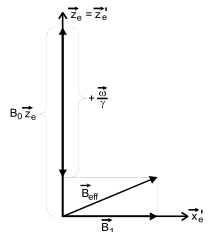
\includegraphics[width=0.3\textwidth]{bfeld.PNG}
  \caption{Effektives Magnetfeld das auf die Probe wirkt. \cite{sample}}
  \label{fig:bfeld}
\end{figure}
\FloatBarrier
Für den Fall $B_0=\frac{\omega}{\gamma}$ entspricht grade $B_{eff}=B_1$
und die $\vec{M}$ dreht sich aus der $\vec{e}_z$-Achse heraus.
Der Drehwinkel $\delta(\Delta t)$ beträgt dabei
\begin{align}
  \delta(\Delta t)=\gamma B_1 \Delta t.
\end{align}
Um die Magnetisierung um $\SI{90}{\degree}$ zu drehen beträgt die
Einstrahlungszeit
\begin{align}
  \Delta t_{90} = \frac{\pi}{2\gamma B_1}.
\end{align}
Die Magnetisierung zeigt somit in die $\vec{e}'_y$-Richtung, dies
entspricht einem $\SI{90}{\degree}$-Puls.
Für einen $\SI{180}{\degree}$-Puls beträgt die Einstrahlungszeit
$\Delta t_{180}=2\Delta t_{90}$ und die Magnetisierung $\vec{M}$
zeigt in $-\vec{e}_z$-Richtung.
Durch Anwenden dieser diskreten Pulse lassen sich
wohldefinierte Nicht-Gleichgewichtszustände erzeugen.
Da die Magnetisierung nach den Pulsen wieder zu dem
Gleichgewichtszustand zurückstrebt, lassen sich so die
Relaxationszeiten $T_1$ und $T_2$ messen.

\subsection{Messmethoden}
\subsubsection{Bestimmung der Relaxationszeit $T_2$}
\paragraph{Freier Induktionszerfall (FID)}
Für einen FID wird die Probe
in ein homogenes Magnetfeld $B_0\vec{e}_z$ platziert.
Zusätzlich befindet sich die Probe in einer
Spule, die senkrecht zu dem Feld steht.
Durch die Spule wird ein hochfrequentes Magnetfeld
mit der Frequenz $\omega_L=\gamma B_0$ eingestrahlt.
Somit können wie in \ref{para:HF} ein $\SI{90}{\degree}$- oder $\SI{180}{\degree}$-Pulse
realisiert werden.
Bei dem freien Induktionszerfall wird die Probenmagnetisierung mit einem
$\SI{90}{\degree}$-Puls in $\vec{e}'_y$-Richtung rotiert. Nach
Abschalten des Pulses
führt die Magnetisierung dann eine Präzessionsbewegung in der
x-y-Ebene auf Grund des noch bestehenden $B_0\vec{e}_z$ Feldes aus.
Die dadurch entstehende Induktionsspannung in der Spule wird in Abhängigkeit der Zeit aufgenommen.
Der Zerfall der transversalen Magnetisierung und somit auch abnehmen der
Induktionsspannung mit der Zeit, besitzt zwei Gründe.
Zum einen existiert kein perfektes homogenes Magnetfeld bei einer
realen Apparatur und zum anderen
existieren Dipolfelder der nächsten Nachbarn und Spins in der Elektronenhülle,
die ebenfalls einen Inhomogenität des Magnetfeldes in der Probe erzeugen.
Die Larmorfrequenzen der einzelnen Spins sind somit nicht mehr für alle Spins
gleich, sondern es existiert eine Verteilung der Larmorfrequenz.
Dies führt zu einer Dephasierung
der Spins, da manche Spins schnell oder langsamer
als mit der Frequenz $\omega=\gamma B_0$ rotieren.
Die transversalen Magnetisierung nimmt deshalb mit der Zeit ab.
Messbar ist nur die Relaxationszeit $T_2^*$
mit
\begin{align}
  \frac{1}{T_2^*} = \frac{1}{T_2} + \frac{1}{T_{\Delta B}}
\end{align}
wobei $T_{\Delta B}$ der Zeitkonstante entspricht, die durch die Inhomogenität
des $B_0\vec{e}_z$ hervorgerufen wird.
Für ein hinreichend homogenes Feld ist $T_{\Delta B} \gg T_2$
und $T_2$ kann mit dem FID bestimmt werden.
Jedoch für $T_{\Delta B}$ \textless $T_2$ ist eine $T_2$-Bestimmung wegen
der apparativen Feldinhomogenitäten über FID nicht mehr möglich.

\paragraph{Spin-Echo-Verfahren}
Die Spin-Echo-Methode bietet eine Möglichkeit die apparativen Störeffekte
bei der $T_2$-Bestimmung zu eliminieren.
Dabei werden mindestens zwei HF-Pulse benötigt.
Mit einem $\SI{90}{\degree}$-Puls wird die Probenmagnetisierung in die
$\vec{e}'_y$-Richtung gedreht.
Wegen der verschiedenen Larmorfrequenzen der einezelnen Spins, beginnt die Dephasierung.
Im rotierendem Koordinatensystem drehen somit Spins mit $\omega_{L_\text{Spin}}<\omega_{Hf}$
gegen und Spins mit $\omega_{L_\text{Spin}}>\omega_{Hf}$ mit dem
Uhrzeigersinn um die $\vec{e}_z$-Achse.
Bereits nach der Zeit $T_{\Delta B}$ ist die transversalen
Probenmagnetisierung durch
Auseinanderlaufen der Spins so gut wie verschwunden,
sodass kaum ein Induktionssignal
gemessen wird. Wird nach dem $\SI{90}{\degree}$-Puls
zum Zeitpunkt $\tau$
ein $\SI{180}{\degree}$-Puls
auf die Probe gegeben, wird nach $2\tau$,
wie in Abbildung \ref{fig:hahn-echo} dargestellt,
das sogenannte Hahn-Echo beobachtet.
\begin{figure}
  \centering
  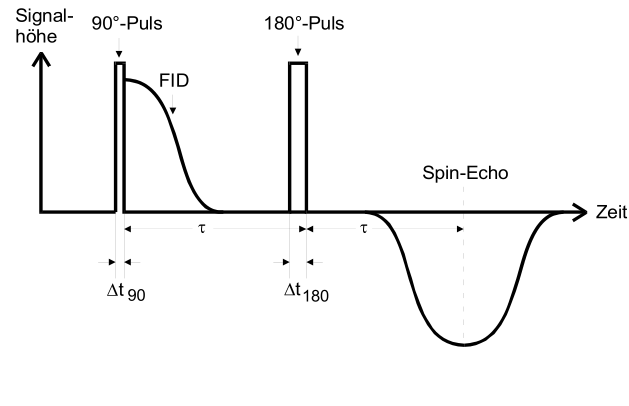
\includegraphics[width=0.7\textwidth]{hahn-echo.PNG}
  \caption{Signalverlauf des Hahn-Echos.\cite{sample}}
  \label{fig:hahn-echo}
\end{figure}
Durch den $\SI{180}{\degree}$-Puls führen
die Spins eine Drehung um die
$\vec{e}'_x$-Achse aus und laufen wieder zusammen
zum Zeitpunkt $2\tau$ sind alle Spins wieder in Phase und eine
transversalen Probenmagnetisierung
erzeugt wieder ein Spignal in der Spule.
Der zeitliche Verlauf der Spins ist in Abbildung
\ref{fig:spin-echo} dargestellt.
\FloatBarrier
\begin{figure}
  \centering
  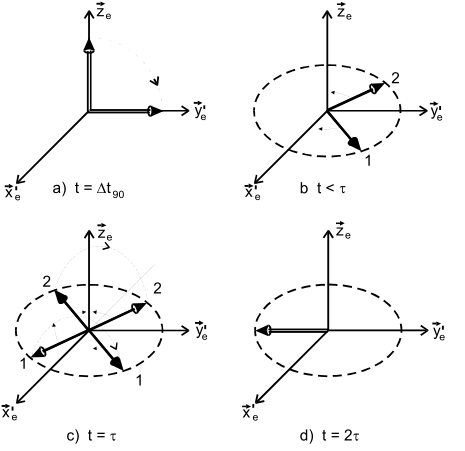
\includegraphics[width=0.6\textwidth]{spin-echo.PNG}
  \caption{Zeitlicher Verlauf der verschiedenen Spinmagnetisierungen während des Hahn-Echos.\cite{sample}}
  \label{fig:spin-echo}
\end{figure}
\FloatBarrier
Das Hahn-Echo-Signal besitzt im Vergleich zum Startsignal
ein anderes Vorzeichen, da die transversale
Magnetisierung zum Zeitpunkt $2\tau$ in $-\vec{e}_y$-Richtung zeigt.
Für $T_2\rightarrow\infty$ erreicht die betragsmäßige
Amplitude des Echos die
ursprüngliche Höhe vor dem FID.
Jedoch treten zu den reversiblen Dephasierungsprozessen auch
irreversible auf wie Wechselwirkung. Diese führen zur Abnahme der Echo-Stärke $M_Y$,
wie in Abbildung \ref{fig:tau_ver} dargestellt,
in Abhängigkeit von der Zeit in der Form
\begin{align}
  M_Y(t)=M_0 \exp\left(-\frac{t}{T_2}\right).\label{eqn:t2}
\end{align}
\FloatBarrier
\begin{figure}
  \centering
  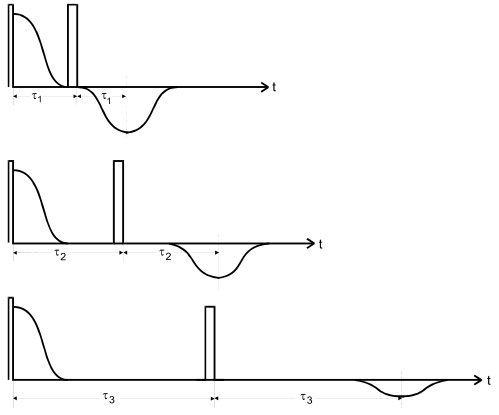
\includegraphics[width=0.7\textwidth]{tau_ver.PNG}
  \caption{Zeitlicher Verlauf des Hahn-Echos für unterschiedliche $\tau$.\cite{sample}}
  \label{fig:tau_ver}
\end{figure}
\FloatBarrier
\paragraph{Carr-Pucell- und Meiboom-Gill-Methode}
Die beiden Methoden liefern im Vergleich zur Spin-Echo-Methode eine
schnellere Möglichkeit der $T_2$-Bestimmung, da während der Messung die Magnetisierung
nicht in die Gleichgewichtslage zurückkehren muss.
Bei der Carr-Pucell-Methode wird ebenfalls ein $\SI{90}{\degree}$-Puls
verwendet jedoch nach dem ersten $\SI{180}{\degree}$-Puls
im äquidistanten Abstand von $2\tau$ weitere $\SI{180}{\degree}$-Puls
auf die Probe gegeben. Der dadurch erzeugte Signalverlauf
ist in der Abbildung \ref{fig:carr-pu} zu sehen.
\begin{figure}
  \centering
  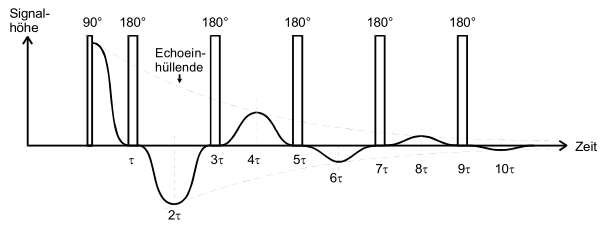
\includegraphics[width=0.8\textwidth]{carr-pu.PNG}
  \caption{Zeitlicher Verlauf des Signales bei der Carr-Purcell-Methode.\cite{sample}}
  \label{fig:carr-pu}
\end{figure}
Durch die aufeinanderfolgenden $\SI{180}{\degree}$-Pulse werden
weitere Hahn-Echos erzeugt und
somit können mit einem Messvorgang mehrere Messpaare von Zeit und
Echoamplitude aufgenommen werden, um $T_2$ durch den Zusammenhang \eqref{eqn:t2} zu bestimmen.
Eine genau $T_2$-Bestimmung gelingt aber nur dann,
wenn die $\SI{180}{\degree}$-Pulse exakt eingestellt sind, da
bei falscher Justage die Magnetisierung mit dem Winkel $\delta$ aus der x'-y'-Ebene
dreht. Weil nur die Komponente die in der x'-y'-Ebene zum Signal beiträgt,
wird dieses zu klein gemessen. Zusätzlich kommt hinzu, dass
sich bei jedem weiterem Puls die Fehler addieren wird.
Somit ergibt sich ein kleineres $T_2$.
Die Meiboom-Gill-Methode hingegen verwendet eine
Pulsfolge, die diesen Fehler reduziert. Dabei wird folgendermaßen
vorgegangen, die $\SI{180}{\degree}$-Pulse bewirken
jetzt eine Dreheung um die $\vec{e}'_y$-Achse und nicht mehr
um die $\vec{e}'_x$-Achse, indem die Phase des HF-Feld
für den $\SI{180}{\degree}$-Pulses zum HF-Feld des $\SI{90}{\degree}$-Pulses
um $\SI{90}{\degree}$ verschoben wird.
Dies hat den Vorteil, dass dadurch bei jeder
gerader Pulsanzahl trotz Drehung
um $\SI{180}{\degree}+\delta$ die Magnetisierung wieder in der x'-y'-Ebene
landet, wie in Abbildung \ref{fig:mei-gil} zu sehen ist.
Die Echoamplitude $M_y$ nach jedem geraden Puls kann somit zu
$T_2$-Bestimmung benutzt werden.
Zusätzlich ist die Amplituden durch die Drehung
um die y'-Achse im Vergleich zur Carr-Purcell-Methode stets positiv.
\begin{figure}
  \centering
  \centering
  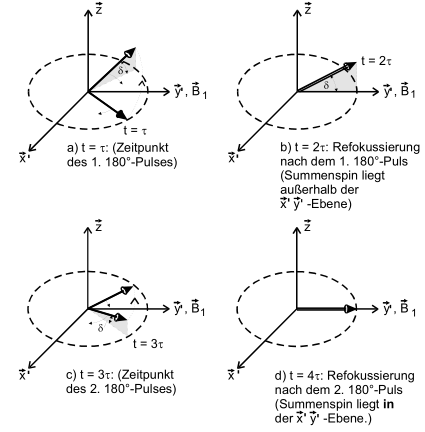
\includegraphics[width=0.6\textwidth]{mei-gil.PNG}
  \caption{Beispiel Verlauf einer Spinmagnetisierung bei
  der Meilboom-Gill-Methode.\cite{sample}}
  \label{fig:mei-gil}
\end{figure}
\subsection{Einfluss der Diffusion auf das Relaxationsverhalten}
Wenn eine Zeitabhängigkeit des lokalen
$B_0\vec{e}_z$-Feldes für die Spins existiert, kann $T_2$ nicht mehr über die Gleichung
\eqref{eqn:t2} bestimmt werden. Dies ist zum Beispiel
durch die Brownsche Molekularbewegung gegeben, da
die Spins in Folge der Inhomogenitäten des statischen Feldes
in Bereiche unterschiedlicher Feldstärken gelangen.
Infolge dessen wird die Larmorfrequenz zeitabhängig
und die Refokussierung der Spins wird gestört.
Somit nimmt die
Signalamplitude stärker als in Gleichung \eqref{eqn:t2}
ab.
Um diese thermischen Bewegungen der Atome/Moleküle
in Flüssigkeiten zu berücksichtigen
werden die Blochschen Gleichungen um eine Term mit der
Diffusionskonstante $D$ erweitert und es ergibt sich
\begin{align}
\frac{\delta\vec{M}}{\delta t} = \gamma\left(\vec{M}\times\vec{B}\right)-\frac{M_x\vec{e}_x+M_y\vec{e}_y}{T_2}-\frac{\left(M_z-M_0\right)\vec{e}_z}{T_1} +(\vec{e}_x+\vec{e}_y+\vec{e}_z)D\Delta M.
\end{align}
Des Weiteren wird einem Feld
\begin{align}
\vec{B}_0= (B_0 + Gz) \vec{e}_z
\end{align}
mit konstantem Feldgradienten $G$ in z-Richtung betrachtet
und die Inhomogenitäten des Feldes in x- und y-Richtung vernachlässigt,
da diese die Larmorfrequenz nur in 2.Ordung ändert.
Wird nun die transversalen Magnetisierungskomponente
$M_{tr}=M_x + \symup{i}M_y$
betrachtet, kann die Gleichung mit dem Ansatz
\begin{align}
  M_{tr} = f(x,y,z,t) \exp\left(-\symup{i}\omega_Lt\right) \exp\left(-\frac{t}{T_2}\right)
\end{align}
gelöst werden.
Dabei muss die Funktion $f$ die Gleichung
\begin{align}
\frac{\delta f}{\delta t} = -i\gamma Gzf + D\Delta f
\end{align}
zusätzlich erfüllen.
Als Ergebnis ergibt sich dann für die Echoamplitude
\begin{align}
M_Y(t)&= M_0\exp\left(-\frac{t}{T_2}\right)
\exp\left(-\frac{t}{T_D}\right) \label{}
\intertext{mit der Zeitkonstanten}
T_D&=\frac{3}{D\gamma^2 G^2 \tau^2}.
\end{align}
Für eine Erfolgreiche $T_2$ Messung muss $T_D$ groß gegen $T_2$
sein. Dies kann durch Variation des frei wählbaren
Parameters $\tau$ erfüllt werden.

Des Weiteren ist es möglich die
Diffusionskonstante mit der Spin-Echo-Methode
zu messen, wenn der Feldgradient $G$ der Apparatur bekannt ist.
Dafür wird $\tau$ variert und die Echoamplitude zum Zeitpunkt $t=2\tau$ bestimmt.
Die Echoamplitude folgt somit der Gleichung
\begin{align}
M_Y(t) = M_0\exp\left(-\frac{t}{T_2}\right)
\exp\left(-\frac{D\gamma^2 G^2 t^3}{12}\right) \label{eqn:32}
\end{align}.
Dies funktioniert, solange
\begin{align}
  T_2^3 \ll \frac{12}{D\gamma^2 G^2}
\end{align}
gilt, da die Zeitabhängigkeit von $M_y$ durch den Diffusionsterm gegeben ist.

\subsection{Bestimmung der longitudinalen Relaxationszeit $T_1$}
\label{subsec:t1}
Zur Bestimmung von $T_1$ werden ebenfalls Pulse verwendet.
Jedoch wird mit einem $\SI{180}{\degree}$-Puls zunächst die Probenmagnetisierung
aus der Gleichgewichtslage in die entgegengesetzte
Richtung gedreht. Die Magnetisierung beginnt danach
wieder zur Gleichgewichtslage zu streben.
Nach einer Zeit $\tau$ wird
die verbliebenen Magnetisierungskomponente in z-Richtung $M_z$
mit einem $\SI{90}{\degree}$-Puls in die x-y-Ebene gedreht.
Diese führt dann eine Präzessionsbewegung aus und induziert eine
Induktionsspannung proportional zu $M_z(\tau)$ in der Spule.
Durch Lösen der Blochschen Gleichung \eqref{eqn:bloch}
mit den Anfangsbedingungen $M_x(0)=M_y(0)=0$ und $M_Z(0)=-M_0$
ergibt sich der Zusammenhang
\begin{align}
  M_z(\tau) = M_0 \left(1 - 2 \exp\left(-\frac{\tau}{T_1}\right)\right). \label{eqn:33}
\end{align}
mit der longitudinalen Relaxationszeit $T_1$ (siehe Abb. \ref{fig:M_z}).

\begin{figure}
  \centering
  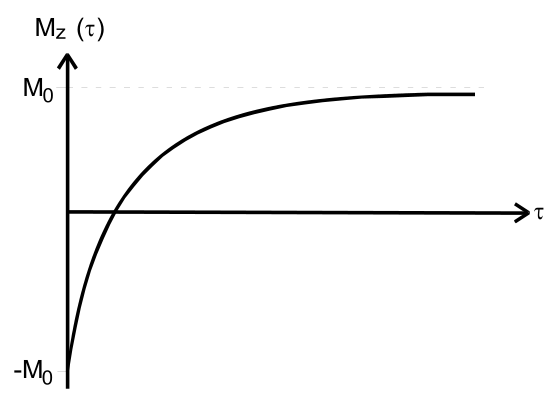
\includegraphics[width=0.5\textwidth]{M_z.PNG}
  \caption{Schematische Verlauf der Magnetisierungskomponente $M_z$
    in Abhängigkeit der Zeitspanne zwischen den Pulsen $\tau$ nach Gleichung \eqref{eqn:33}.\cite{sample}}
  \label{fig:M_z}
\end{figure}
% test
%
% \subsection{Messmethoden}
% \paragraph{Spin-Echo-Methode}
% \paragraph{Carr-Pucell-Methode}
% \paragraph{Meiboom-Gill-Methode}
